% !TEX root = HowToRobot.tex

\chapter{Electrical Design}
\label{chap:ElecDes}

\section{Design Considerations}
Another important aspect of your robot is ensuring that it is electrically capable of fulfilling requirements - and making sure it doesn't light itself on fire or electrocute anyone. The best mechanical design in the world is useless if there's nothing to supply power to the wheels, and your computer is just a hunk of plastic and metal if it doesn't get the right amount of power. While electrical design for a robot is not very complicated (unless you want it to be), it does require some fundamental knowledge.

\subsection{The Basics}
We'll start off easy. I'm going to restrict the discussion here to (relatively) low voltage DC circuits. Within that domain, there are three very important terms. Voltage, measured in Volts (V), Current, measured in Amperes "Amps" (A), and Resistance, measured in Ohms $\Omega$. A very smart German dude by the name of Georg Ohm came up with probably the most important (for us at least) law in all of electronics back in 1827, and published it in his book \textit{Die galvanische Kette, mathematisch bearbeitet}. (Translated to English, that's \textit{The Galvanic Circuit Investigated Mathematically}). The book is available online, but I wouldn't recommend it unless you're in for some heavy reading. It was written in the early 1800s after all. The important part - the law we care about here - is called Ohm's law and is shown in Equation \ref{eqn:ohmslaw}.

\begin{equation}
V = IR
\label{eqn:ohmslaw}
\end{equation}

That's it. That's all there is to it. Voltage (V) equals Current (I) times Resistance(R). This law has the interesting property that, unlike everything else we do in Electrical Engineering, it almost always holds true. So, if something isn't behaving the way you think it should, refer to this law.

Ok, so now we have the fundamental law of the universe, but so what? What are all these funky terms? Let's talk more about that. Sparkfun also has a pretty excellent page explaining this, so if my explanation doesn't work out for you, just search for \textit{Sparkfun Voltage, Current, Resistance, and Ohm's Law}.

\subsection{Voltage}
Voltage behaves very much like water pressure in a pipe. With water, pressure - or more accurately, pressure differential - is what causes water to flow. However, just because there is pressure doesn't mean the water actually flows. It's just a measure of how much the water \textit{wants} to flow. For example, consider a completely full, sealed container of water. Now shrink the volume of the container by half without letting any water out. Some laws that I vaguely remember from chemistry say that the pressure has to increase. (Or temperature, but we're going to ignore that bit). Now there's more pressure, but the container is still sealed with no route for the water to escape, so there's no flow.

Voltage behaves almost exactly the same. Except instead of water, we have a high density of electrons. Because they are negatively charged, and like charges repel one another, electrons like to spread out as much as they can to reach the minimum energy configuration. Sort of like when you drop a glass of water on the floor, and the water spreads out to get as low to the ground as possible - thereby reducing it's gravitational potential energy and reaching a minimal energy state. So, compressing a lot of electrons in to a small space creates this electrical pressure - voltage, or "electromotive force" for people who like words with many syllables.

The common source of voltage differentials in mobile robotics are batteries or DC power supplies.

\subsection{Current}

If voltage is pressure, than current is the amount of flow. If there is a pressure differential, and a route for water to escape, then flow happens in a pipe. This flow continues until the pressure differential is balanced out. Batteries work the same way. (By the way, think of power supplies as infinite batteries.) A fully charged battery has some voltage, and if there is a path from the negative terminal to the positive terminal, electrons will flow along that path. As the electrons flow from negative to positive and thereby "spread out" to the minimal energy state, the battery voltage will decrease. This flow is current.

\subsection{Resistance}

Resistance is not a property of the electricity itself, but a property of the material it flows through. The easy analogy is to think of the resistance as the size of the pipe. A narrower pipe allows less water to flow through. Likewise, a material with higher resistances "resists" the flow of electrons more strongly. In low power DC applications, you can generally assume that wires have a resistance of 0.

Often, we will use components called "Resistors" to purposefully introduce resistance in a circuit. This is particularly useful when we have components like LEDs (light-emitting diodes) which can only handle so much current. We'll have an example circuit a little later demonstrating how to choose the right resistor for an LED.

There is one more thing you need to know about resistors before we move on. What happens if you have more than one? There are two ways to hook up multiple resistors. You can put them in parallel or in series. Figure \ref{fig:resistorscombinations} shows both configurations. When resistors are hooked up in series, the value of the resistors just adds up, so you can pretend like you have one big resistors with a value that is the sum of all the resistors in series. For completeness, this is shown in Equation \ref{eqn:seriesresistors}. When resistors are hooked up in parallel, the resistance of the set of resistors actually decreases. I'll explain why a bit more intuitively in the next section, but the math for calculating the resistance of a set of parallel resistors is shown in Equation \ref{eqn:parallelresistors}.

\begin{equation}
R = R_1 + R_2 + \cdots + R_n
\label{eqn:seriesresistors}
\end{equation}

\begin{equation}
\frac{1}{R} = \frac{1}{R_1} + \frac{1}{R_2} + \cdots + \frac{1}{R_n}
\label{eqn:parallelresistors}
\end{equation}

\begin{figure}
\centering
\begin{subfigure}{.5\textwidth}
  \centering
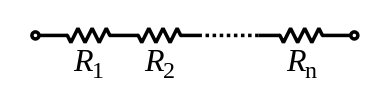
\includegraphics[width=\textwidth]{seriesresistors.png}
  \caption{Series}
  \label{fig:seriesresistors}
\end{subfigure}%
\begin{subfigure}{.5\textwidth}
  \centering
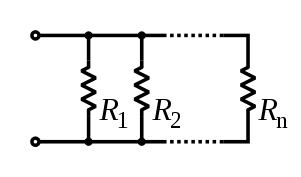
\includegraphics[width=.5\textwidth]{parallelresistors.png}
  \caption{Parallel}
  \label{fig:parallelresistors}
\end{subfigure}
\caption{Resistor Combinations}
\label{fig:resistorscombinations}
\end{figure}


\subsubsection{Putting It All Together}

Example time! First, look at the picture in Figure \ref{fig:parallelresistorsexample}. In that example, there are multiple paths for the electricity to follow. Meditating on Ohm's law for a while will eventually lead you to the mathematical reason behind this, but for now just take my word for it: the electricity divides itself up among the possible paths inversely proportional to the resistance of each path. Ohm's law requires this, and it's actually convenient for us because it generates the least possible waste heat - but that's an advanced topic I won't cover here. Let's attach some real numbers to this example. Consider a circuit with a 10V voltage source and 2 resistors in parallel, one 5$\Omega$ and one 10$\Omega$. This example circuit is shown in Figure \ref{fig:parallelresistorsexample}. Reducing the two resistors with Equations \ref{eqn:parallelresistors}, gives the circuit showin in Figure \ref{fig:parallelresistorsexamplemerged}.


\begin{figure}
\centering
\begin{subfigure}{.5\textwidth}
  \centering
  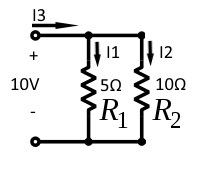
\includegraphics[scale=0.75]{parallelresistorsexample.png}
  \caption{Parallel Resistors}
  \label{fig:parallelresistorsexample}
\end{subfigure}%
\begin{subfigure}{.5\textwidth}
  \centering
  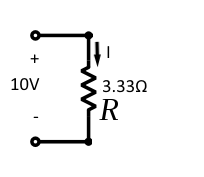
\includegraphics[scale=0.75]{parallelresistorsexamplemerged.png}
  \caption{Reduced}
  \label{fig:parallelresistorsexamplemerged}
  \end{subfigure}
\caption{Parallel Resistor Example}
\label{fig:resistorscombinations}
\end{figure}

There are a few things to think about in this example. First, note that I3 in Figure \ref{fig:parallelresistorsexample} must be equivalent to the current I in Figure \ref{fig:parallelresistorsexamplemerged} since they are in truth the same circuit. In Figure\ref{fig:parallelresistorsexamplemerged}, we can easily solve for I using Ohm's law.

\begin{equation} \label{eqn:solvefori}
\begin{split}
V = IR \\
10 = I(3.33)\\
I = 10/3.33 \\
I = 3A
\end{split}
\end{equation}


We can likewise solve for I1 and I2 in Figure \ref{fig:parallelresistorsexample} using the same manner, but with R values of 5$\Omega$ and 10$\Omega$ respectively. This gives us I1 = 2A and I2 = 1A. Notice that I3 = I1 + I2. Another side-effect of Ohm's law is that the sum of all currents entering and leaving a node is 0, which is intuitive if you think about it. It's the same thing as splitting a hose. The sum of the volumes of water that come out of the two hoses must be the same as the volume that goes in to the un-split end.

\subsection{Blinking Lights}

One of the first things most people want to do with circuits is make lights blink. This is good. In the micro-controller world, you often don't have a terminal output until after you get through a decent amount of setup, so blinking LEDs can be the only way to debug problems during boot. The first thing most people do when they want to blink a light is blow one up. This should generally be avoided, although LEDs are cheap and it's a good learning experience.

First, let's look at the proper way to hook up an LED, shown in Figure \ref{fig:ledcircuit}. The main thing to note here is the resistor. Supplying too much current to an LED lets out the magic smoke, and remember, if you let out the magic smoke, the component no longer works. The next question, is how do you choose a value for R? This depends on the LED, and the voltage source. For kicks, let's assume you've got a 5V power supply, from an arduino GPIO for example. By the way, drawing too much power from an arduino GPIO is a good way to kill it, although the LED usually goes first. I'll assume you've got an LED that wants 10mA of current, although this may vary. Check the datasheet for your specific part.

There is one caveat about LEDs. We haven't talked about diodes because it's out of the scope of this document. However, LEDs are a special type of component called a "semi-conductor" which means it is only conductive some of the time. In this case, the LED is only conductive when it has at least a certain threshold of voltage pushing in the "correct" direction. Pay attention to which side the Anode and Cathode of your LED are plugged in to. If it's in the wrong way, current will not flow. (Unless you supply enough voltage to cause the diode to enter the "breakdown" voltage region. In this case, that's the amount of voltage where the LED breaks, but the breakdown region is actually very important for some components. Google "Zener Diode" for more on that. Hint: They're used in motor driver boards for back-emf protection.)

So why do we care about the LED being a semi-conductor? Because semi-conductors usually have a property called a "voltage-drop". This property causes the component to eat a portion of the voltage in the circuit. Your LED datasheet should say something about the voltage drop of the LED, but a typical value is 0.7V for hobby level LEDs. We typically model this voltage drop as a small voltage source pointed in the "wrong" direction. See Figure \ref{fig:ledcircuitvoltagedrop}.

\begin{figure}[h]
\centering
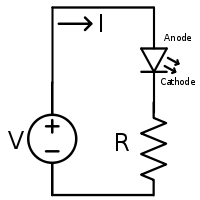
\includegraphics[scale=0.75]{ledcircuit.png}
\caption{LED Proper Hookup}
\label{fig:ledcircuit}
\end{figure}

\begin{figure}[h]
\centering
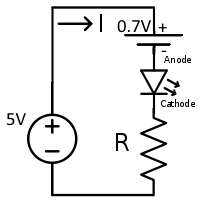
\includegraphics[scale=0.75]{ledcircuitvoltagedrop.png}
\caption{LED Proper Hookup - With Voltage Drop}
\label{fig:ledcircuitvoltagedrop}
\end{figure}

In this case we can just sum the two voltage sources, and pretend we have a 4.3V power supply. So, we have a 4.3V source, and we want a 10mA current. Easy, right? Just use Ohm's law as shown in Equation \ref{eqn:findledr}.

\begin{equation} \label{eqn:findledr}
\begin{split}
V = IR \\
4.3 = (.01)R\\
R = 4.3/.01 \\
R = 430\Omega
\end{split}
\end{equation}

It so happens that LEDs are generally pretty robust. You can probably go plus or minus about 50\% on that R value. A smaller value with make the LED brighter, while a larger value will make it dimmer. Giving and LED too much current will burn it out. An excessively large amount of current \textit{may} make it explode. I highly recommend trying it once under controlled circumstances. Wear eye protection! There will probably be exactly one or two pieces of shrapnel, but it would really suck to get one in your eye. For best results, connect the LED to a power supply and slowly turn up the voltage (starting from 0). You'll get to see all phases of operation for the LED. Below 0.7V it probably will not turn on. From 0.7 to somewhere around 4-6V it will steadily get brighter. At some point it will reach a maximum brightness and then begin to heat up, at which point it will probably start to dim. At some point after that, it will go out. Cranking up the voltage more will (probably) cause it to explode. 

Note: It is generally not a fiery explosion, so eye protection is generally sufficient precautions.

Note 2: No, that's not a challenge. If you light the lab on fire trying this then you did it on purpose. Consider yourself warned and thus fully liable for any damage you cause.

Sometimes the conductive element inside just melts and you don't get an explosion. It really depends on the LED.

\subsection{Voltage Divider}

There's one last circuit I want to mention because it becomes very important when dealing with analog sensors. The voltage divider. An example is shown in Figure \ref{fig:voltagedivider}. The basic idea here is that you have a known resistor value for R1, and some variable value for R2. A common one is a thermistor - a resistor that changes its value based on temperature. In fact, an excellent experiment to try is to use a thermistor in exactly this circuit configuration to measure the temperature of water. It's very easy, and will teach you about the analog to digital converter. It will probably also teach that water is conductive, and shortly thereafter that hot glue is not (for electricity or heat). There's also the matter of sensor calibration, but I won't go in to the details on that here. Suffice it to say that all sensors are terrible, and you should never trust them until you've tested them rigorously.

\begin{figure}[h]
\centering
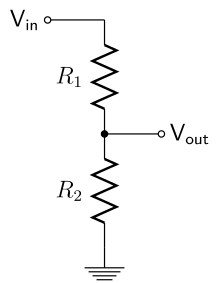
\includegraphics[scale=0.75]{voltagedivider.png}
\caption{Differential Drive}
\label{fig:voltagedivider}
\end{figure}

The general plan is to supply a known voltage to $V_{in}$, have a known $R_1$, and measure $V_{out}$. With these pieces of information, you can solve for $R_2$ using Ohm's law. The derivation isn't difficult, but other people have already done it, so here it is. Once you have $R_2$ you just refer to your sensor calibration or the datasheet for the part, and you have your value for (in this case) temperature.

\begin{equation} \label{eqn:solveforr}
\begin{split}
R_2 = R_1*\frac{1}{(\frac{V_{in}}{V_{out}}-1)}
\end{split}
\end{equation}

\section{Batteries}
\label{sec:batteries}

\subsection{The Basics}

We have had a lot of problems dealing with batteries over the years. Partly because people are lazy, but mostly because they don't understand how batteries work or how to properly maintain them. All batteries are basically slow, controlled, chemical reactions. They are not magical devices that store and dispense electric charge. The closest thing to that is a capacitor, which is two metal plates with an insulator between them. By applying voltage, you charged the plates, storing energy in the form of actual electric charge. However, capacitors tend to discharge all of their stored energy at once. In adddition, the total energy they can store is far less than most batteries. Batteries, on the other hand, store energy in the form of chemical potential energy. This is far more stable than storing raw electric charge, but it does lead to a few problems. The big one is that, since the energy storage relies on chemistry, temperature is important. Being stored in a place that is too hot or too cold can cause a battery to burst, or drain it. Another is that, over time, the chemistry can get disrupted, causing the battery's maximum storage potential to decline.

\subsection{Which Numbers Are Important?}

Now you know what voltage, current, and resistance all mean, but how do you use them in practice? 

\subsubsection{Voltage - V}

We'll start with voltage because that's the easiest one to handle. You want to make sure the voltage your batteries produces matches the voltage rating for the things you want to power: motors, cpu, sensors, etc. However, there's another consideration to make. You almost never want your batteries directly connected to your sensitive electronics. You always want a regulator of some sort in between. Why? As you drain a battery, the voltage will decline over time. In addition, large loads on the battery can temporarily cause the voltage to fluctuate i.e. powering motors. Motors also cause back-emf, but we'll talk about that later. All of this can cause damage to unshielded electronics. We'll talk about regulators in Section \ref{sec:regulators}. In addition to the power fluctuations, you rarely have motors that you want to drive with the same voltage as the computer. In practice, you'll want to match your main battery voltage to the voltage of the motors you want to power, and then use regulators to smooth and reduce the voltage for the other components.

\subsubsection{Capacity - mAh "milli-Amp Hours"}

This is the best measure of how much actual energy the battery can hold. To put it simply, a 1000mAh battery could sustain a drain of 1A for 1 hour before being depleted. If you draw 2A it will only last half an hour. At 0.5A, two hours. It's a very silly unit when you think about it, but it makes the math easy.

\subsubsection{C}

Most batteries have a C rating. This is a somewhat cryptic value that tells you how quickly a battery can discharge without damaging itself. This is not a limit on how much current the battery can draw. Remember Ohm's law? You thought it wasn't important, didn't you? The thing is, Ohm's law will dictate the current that gets drawn from the battery. The C rating just tells you what is safe. The tricky bit is that the actual safe rate of discharge depends on the size of the battery. Weird right? Here's the simple way to think about it. The amount of continuous current drain a battery can handle without damaging itself is obtained by multiplying the C rating with the battery capacity. For instance, a 1500mAh battery with a 5C rating can handle a continuous drain of 30,000mA or 30A.


\subsection{Lead Acid Batteries - Pb}

Lead acid batteries are very stable. That's why we use them in cars. They also have a pretty good capacity, and are able to source a tremendous amount of current at once. This is good, because it takes a lot of force to turn over an engine. For a rugged, outdoor robot that may experience a variety of temperature conditions, lead-acid may be the way to go. However, lead-acid batteries are generally larger and heavier than their counterparts. Charging them is easy. Just hook them up to a power supply, set the power supply to the battery's rated voltage, and limit the current. What you limit the current to depends on the battery. Car batteries can generally handle up to 6A. The real problem is heat. If you charge too fast, the metal plates in the battery heat up, and can cause the acid to boil. This creates potentially toxic vapors and, if the vapors escape the battery housing, reduce the lifespan and charge of the battery. Other than charging too quickly, there isn't much to worry about here. Please charge in a well-ventilated area, just in case. Running a lead-acid battery dead isn't really a big deal as long as you don't leave it dead for a long time, or it doesn't get too cold while dead.

\subsection{Lithium Polymer - LiPo}

In the robots I built during my time on the team, we used these most commonly. They are light-weight, small, and can store a great deal of power. A LiPo battery generally consists of some number of cells. Each cell has a rated voltage of 3.7V. Batteries with more voltage are built by putting multiple cells in series. This voltage has to do with the internal chemistry. LiPo batteries are not nearly as stable as lead acid. There are three major concerns when dealing with a LiPo. First, only charge using a LiPo charger. There are some extra pins on a LiPo battery that tell the charger important information about the cells within. Second, make sure you look up the rating for charging a LiPo. The general rule of thumb is that a LiPo can be charged at the rate of 1C. If you have a 1500 mAh battery, you can charge it at 1.5A. Charging it slower is fine. Charging faster can cause the LiPo to heat up, swell, and potentially burst. When the LiPo bursts, the chemicals inside will spontaneously burn, creating fire, pressure, and heat. Seriously bad news. Third, never ever cut or puncture a LiPo. An externally ruptured LiPo is bad news, but one that ruptures internally, or without a good pressure relief, is a thermal grenade.

That all said, LiPo batteries are pretty safe if you follow the guidelines I set out for charging. There are two more things to worry about. 3.7V is the rated voltage for a cell, but when you charge, you generally charge to about 4.2V - the charger will handle this. Never manually overcharge the LiPo. However, unlike a lead-acid battery, letting the charge get too low in a LiPo will permanently damage it. The minimum safe level for a single cell is 3V. Always monitor the voltage of LiPo batteries you are using and ensure they don't drop below this level. The difficult part is, LiPo voltage doesn't drop linearly. Figure \ref{fig:lipovoltage} shows voltage versus charge for a LiPo. As you can see from the graph, you have to monitor the battery voltage very carefully, because it decreases rapidly once the charge gets low.

\begin{figure}[h]
\centering
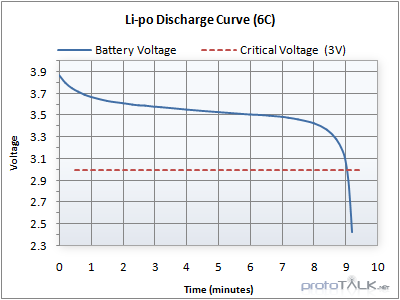
\includegraphics[scale=0.75]{lipovoltage.png}
\caption{LiPo Voltage VS Charge}
\label{fig:lipovoltage}
\end{figure}

As a side note, this chart is for one specific battery I found on a forum post at Traxxas.com. Individual results may vary in specifics, but the point is the same. Monitor your voltage and don't let it drop below 3.0V per cell. There is one additional caveat. LiPo batteries don't hold their charge forever, and they will, if left sitting on a shelf for long periods of time, eventually degrade. It is recommended to discharge and charge a LiPo battery every few months when it is not in active use. Discharging can be done by using the LiPo while closely monitoring the voltage, or with a dedicated charger. The chargers in the lab have this capability.

The final thing to mention is balancing. Because a LiPo battery may be made up of multiple cells, the total voltage isn't enough to tell the health of the battery. In the lab we have at least two balancers. Some chargers will also balance while they charge. Balancing slowly bleeds charge from one cell and puts it into another cell. This keeps the cells from becoming unbalanced. This is a good thing. Each cell may discharge differently because chemistry is a sloppy science and never works quite the way it's supposed to. This can lead to one cell with a much higher or lower voltage than the others. If one cell gets overcharged, it may swell and/or rupture. If one cell gets too low, it may "die". Dead cells are ones that have dropped to a low enough voltage that they cannot safely be recharged. Most chargers will refuse to charge the battery if there are dead cells. If you know what you're doing, sometimes dead cells can be nursed back to life, but it's a delicate and potentially dangerous procedure. It's usually better to recycle the battery and get a new one.

\subsection{Other Batteries}

There are three more common types of batteries. Lithium Iron Phosphate - LiFePO4 often pronounced "LieFo" - Nickle Metal Hydride - NiMH - and Nickle Cadmium - NiCd "Nigh-Cad". I haven't personally worked with these, so the internet is a better resource then I am. My vague understanding is that LiFePO4 are similar to LiPo batteries but more stable and more expensive. A quick Google search tells me that NiMH is the new NiCd, and is used in general consumer electronics, so it must be pretty stable, but doesn't (in general) have as much energy density as Lithium batteries.

\section{Tips For Not Lighting Things On Fire}

Forethought and attentiveness are key for keeping the magic smoke inside the components. All electrical components are made using plastic, silicon, some trace metals, and a mystical substance called magic smoke. If you give the component too much voltage, current, or heat the magic smoke will use this extra energy to break free and escape. It is a very clever substance, and even just a momentary spike is enough to free it. At this point the component will no longer work. Nobody is perfect, but here are a few tips I've picked up over the years to keep the magic smoke locked up tight.

\subsubsection{Turn Off The Power}

This should be common sense, but you'd be surprised how often people get overconfident about what they're doing and modify a circuit while it's powered. Sure, if you know what you're doing you're theoretically safe. The real problem arises when one of those tiny wires gets away from you. Powered wires appear to be supernaturally attracted to conductive terminals, particularly ones that will causes sparks. Just don't do it. The five seconds it takes to flip off the power could save you three days of waiting for new parts.

\subsubsection{Electrical Tape}

If you're working on a circuit, if you aren't immediately dealing with a wire, tape the end. Most of the instances in which I blew something up were because I forgot about a wire that wasn't connected, and it brushed up against something else, making a short. This is particularly important when dealing with batteries. Remember, you can't turn a battery off. If both terminals of a battery aren't connected to something, the free wires should be taped over.

Fun Fact: If you plug the gate pin on a MOSFET in to 24VDC, while the source is floating and the drain is grounded, it explodes. Guess how that happened? I sure didn't plug the gate in to 24VDC on purpose.

\subsubsection{Be Careful Around Batteries}

I've alluded to this several times, but I'll say it again. Always be careful around batteries. I had six years of robotics team experience, and four years of that was while taking courses in Electrical Engineering. At the end of my last semester, I was putting different connectors on some LiPo batteries. I thought to myself, "I'll just cut both wires on the battery at the same time so they'll be the same length."

Technically speaking, it worked out. Turns out the reflex when you hear a loud SNAP and see a bright flash of light is to close your fist, which for me finished cutting the wires and yanked the tool away from the battery cables. It could have been worse though. Just think about what you're doing around batteries. Remember, they can't be turned off.

\subsubsection{Don't Work When You're Tired}

Or drunk. Or sick. Or angry. It makes you inattentive, and then things like the above happen. It doesn't matter how smart you are. Tired people make mistakes.

\subsubsection{Ground Loops}

Ground loops are tricky devils. Explaining the whole mechanism behind them is outside the scope of this document, however, if you are ever dealing with a circuit with multiple power sources, look them up. A ground loop can ruin your whole day. Essentially, ground loops occur when two things you consider "ground" have some resistance between them. If that happens, current through one loop induces a voltage difference in the other loop. Wikipedia is your friend here. Moral of the story - use isolated power supplies, and be very careful when plugging multiple power sources in to one set of electronics. When in doubt, unplug your computer from the wall before plugging anything grounded into it. USB cables, for instance.

\subsubsection{Use the Mult-Meter}

The multi-meter is your friend. When powering up a system for the first time, unplug all sensitive electronics, power the system, and check voltages at your main terminals. Make sure the value \textit{and} the polarity are correct. Then power down, plug in just one piece of equipment, and power back up. Repeat until everything is plugged in. This is useful for two reasons. First, if you have a problem, it will be very obvious which piece is the culprit. Second, if something blows, you risk damaging the minimum possible number of expensive items.
